%%%%%%%%%%%%%%%%%%%%%%%%%%%%%%%%%%%%%%%%%%%%%%%%%%%%%%%%%%
% future work
%%%%%%%%%%%%%%%%%%%%%%%%%%%%%%%%%%%%%%%%%%%%%%%%%%%%%%%%%%

One of our main concerns is that our scripting system as presented so far is aimed at technical users. While this definitely offers advantages, since the game engine itself can be partially coded with scripts to the great benefit of the productivity of developers, the need for less technically inclined users such as designers to access the scripting system is very relevant. After all, designers play a very important role in shaping the behaviors and scripts of a game.

For this reason we are studying a visual editor that allows to create scripts without having to write source code. This editor (which is still a work in progress) would allow the user to drag blocks that represent operations and combinators of our scripts, and assemble them in a fashion that is similar to that of flow-charts.

One of the scripts that we have seen above:

\begin{lstlisting}
(game_over x => ending x) .|| (logic x |> repeat_)
\end{lstlisting}

Would appear in our editor as:

\begin{center}
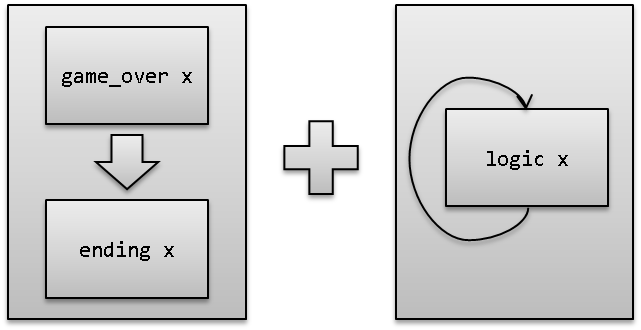
\includegraphics[scale=0.5]{visual_script.png}
\label{Visual script}
\end{center}
